%%%%%%%% ICML 2018 EXAMPLE LATEX SUBMISSION FILE %%%%%%%%%%%%%%%%%

\documentclass{article}


% Recommended, but optional, packages for figures and better typesetting:
\usepackage{microtype}
\usepackage{graphicx}
%\usepackage{subcaption}
\usepackage{subfig}
\usepackage{booktabs} % for professional tables

\usepackage{wrapfig}

% hyperref makes hyperlinks in the resulting PDF.
% If your build breaks (sometimes temporarily if a hyperlink spans a page)
% please comment out the following usepackage line and replace
% \usepackage{icml2018} with \usepackage[nohyperref]{icml2018} above.
\usepackage{hyperref}

% Attempt to make hyperref and algorithmic work together better:
\newcommand{\theHalgorithm}{\arabic{algorithm}}

% Use the following line for the initial blind version submitted for review:
%\usepackage{icml2018}


% If accepted, instead use the following line for the camera-ready submission:
\usepackage[accepted]{icml2018}


% The \icmltitle you define below is probably too long as a header.
% Therefore, a short form for the running title is supplied here:
\icmltitlerunning{Gaussian Processes and CNNs: The utility of Prediction Variance}

\setlength{\textfloatsep}{15pt}

\begin{document}

\twocolumn[
\icmltitle{Gaussian Processes and CNNs: The utility of Prediction Variance}

% It is OKAY to include author information, even for blind
% submissions: the style file will automatically remove it for you
% unless you've provided the [accepted] option to the icml2018
% package.

% List of affiliations: The first argument should be a (short)
% identifier you will use later to specify author affiliations
% Academic affiliations should list Department, University, City, Region, Country
% Industry affiliations should list Company, City, Region, Country

% You can specify symbols, otherwise they are numbered in order.
% Ideally, you should not use this facility. Affiliations will be numbered
% in order of appearance and this is the preferred way.


\begin{icmlauthorlist}
\icmlauthor{Joshua Send}{to}
\end{icmlauthorlist}

\icmlaffiliation{to}{University of Cambridge}

\icmlcorrespondingauthor{Joshua Send}{js2173@cam.ac.uk}


% You may provide any keywords that you
% find helpful for describing your paper; these are used to populate
% the "keywords" metadata in the PDF but will not be shown in the document
\icmlkeywords{Machine Learning, ICML}

\vskip 0.3in
]

% this must go after the closing bracket ] following \twocolumn[ ...

% This command actually creates the footnote in the first column
% listing the affiliations and the copyright notice.
% The command takes one argument, which is text to display at the start of the footnote.
% The \icmlEqualContribution command is standard text for equal contribution.
% Remove it (just {}) if you do not need this facility.

%\printAffiliationsAndNotice{}  % leave blank if no need to mention equal contribution
\printAffiliationsAndNotice{} % otherwise use the standard text.

\begin{abstract}

Convolutional neural networks (CNNs) have long been used to achieve high classification accuracies on a huge variety of tasks. However, they struggle provide information beyond class probabilities, which have to be accepted at face value. Gaussian processes (GPs) are fully Bayesian constructs which can be used to predict both class probabilities and variances for those probabilities, indicating confidence. Using MNIST and related datasets, this paper investigates the effectiveness of combining GPs with CNNs, considering variance for interpretation of results, and as a tool for merging predictions from the base CNN and the GP. This merging process is shown to slightly increase test set accuracy in non-adversarial settings, and points towards future research directions. 

\end{abstract}

\section{Introduction}

%TODOS
%* Discuss how we inevitably will get high probability predictions for junk inputs. Idea: add a "other" class? (and generate a training set for this adverserially/maximize its "reach" somehow?)




\label{sec:intro}

%* Introductory paragraph
% * Problem with CNNs predictions
% * How GPs are bayesian predictors that give variance
% * This work combines ... by ... showing ... (or something)
% * "Interpretable ML"
 
Convolutional Neural Nets (CNNs) have seen a steep rise in use for a wide range of computer vision and machine learning tasks since Krizhevsky's success at the ImageNet challenge in 2012~\cite{krizhevsky2012imagenet}. Given enough training data, they excel in domain specific applications and are efficient to train, but may confidently mis-predict classes, provide no feedback to users about variability of predictions, and have been shown to be vulnerable to adversarial attacks~\cite{szegedy2013intriguing}. On the other hand, Gaussian processes are capable of classification and providing a variance about the prediction. This can be interpreted as a confidence in the probability of a prediction.

This work combines CNNs with Gaussian Processes (GPs), using features extracted by the CNN as input to a GP. This combination takes advantage of neural networks' ability to approximate high dimensional data efficiently and reduce it to a lower dimensional representation; GPs can then produce Bayesian uncertainty estimates along with predictions.

The goal of this work is to explore how useful the variance produced by a GP is, discussing how it might be useful to users, and in enhancing prediction accuracy. Focus will be on image classification using the MNIST~\cite{lecun1998gradient} and N-MNIST~\cite{basu2017learning} datasets, along with adversarially perturbed MNIST images.


\section{Background}
\label{sec:background}
\subsection{Convolutional Neural Nets}
\label{sec:background:cnn}

CNNs are normally used for classification. The following \textit{softmax} activation is applied to the final layer to convert activations into probabilities:

\[ \sigma(z)_j = \frac{e^{z_j}}{\sum_{k=1}^{k=m}e^{z_j}} \]

Combined with categorical-cross entropy loss during training, the resulting values between 0 and 1 from each of the $m$ units represent the posterior distribution over the classes \cite{bridle1990probabilistic}. In other words, we obtain the probability of any class using a fully connected softmax layer. Note that this method reinforces large values and squashes small ones due to the exponentiation, exaggerating differences between classes and not taking into account absolute activation prior to the softmax. 

\subsection{Gaussian Processes}
\label{sec:background:gp}
Gaussian processes are non-parametrized models of functions, defined by a mean and covariance function. The latter determines how related two points in space are -- generally the further away, the less related. The covariance function is built out of a set of \textit{kernels}, and generates a covariance matrix. By incorporating the mean and covariance functions, along with training data, GPs predict both a mean and a variance when given input points. For a simplified example see Figure \ref{fig:gp:basic}.

\begin{figure}[htb]
\centering
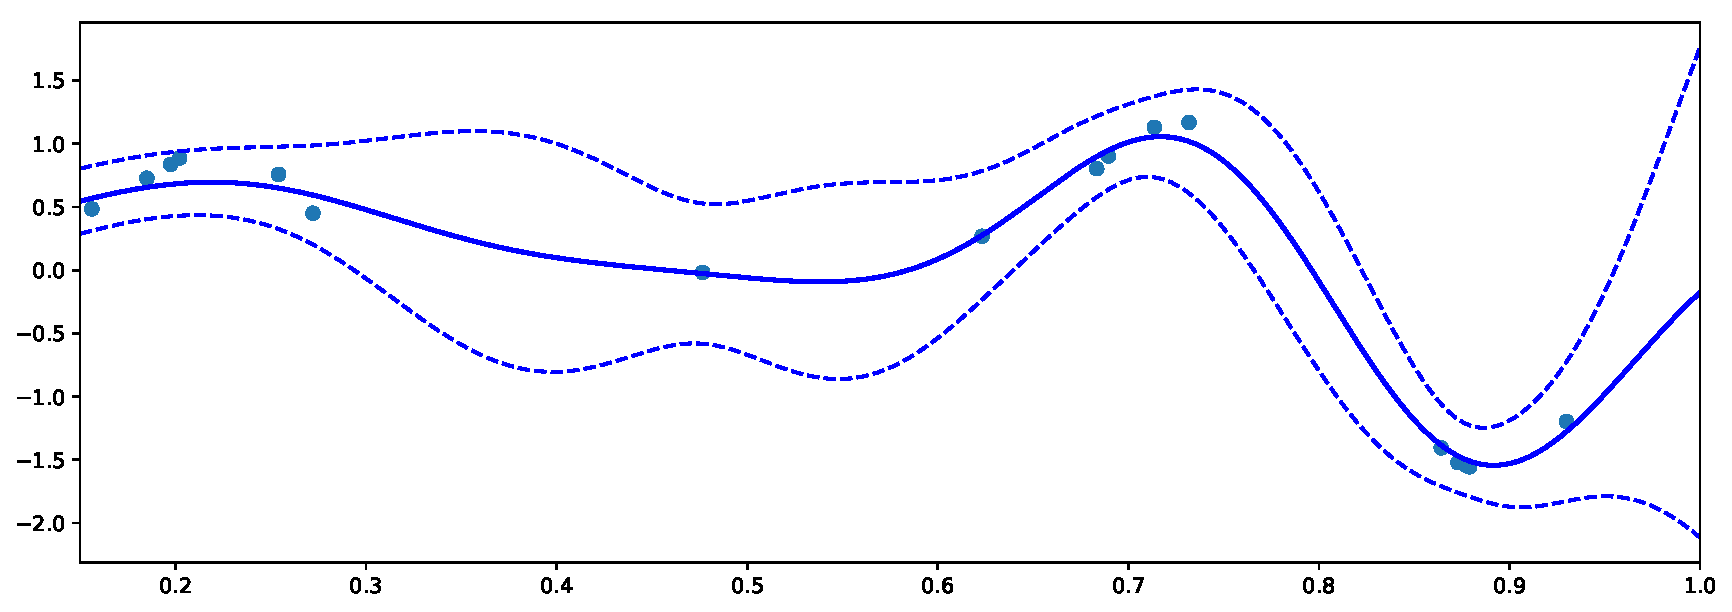
\includegraphics[width=\hsize]{figures/gp_basic.pdf}
\caption{A simple one-dimensional GP regression. The dashed lines represent two standard deviations from the mean, and blue points are training data. Notice how the variance increases away from known datapoints.}
\label{fig:gp:basic}
\end{figure}

By design, trained Gaussian processes have lower variance around known data, while moving away from these points results in much higher uncertainty. This is the property we are most interested in exploiting: when the variance is high, we are in a relatively unknown region of the input space and should put little trust into the predictions.

Another key benefit of GPs is that little hyperparameter tuning is needed -- since the model is fully Bayesian, parameters can be learned directly by maximizing marginal likelihood. However, traditional GPs are costly to train -- covariance matrices are $O(n^2)$ in size, and inversion and decomposition operations have an $O(n^3)$ cost, where $n$ is the number of training samples.

To deal with the issue of scalability\footnote{The training data here is a 60000x128 vector which is formed into a square matrix, far exceeding what could fit into memory}, various approximation methods have been developed. One approach that is used here is called Sparse Variational Gaussian Processes \cite{hensman2015scalable}. This classification approach effectively uses a set of \textit{inducing points} optimized from the training data as an estimate of the full data set; these are then used to fit a GP.

Gaussian processes classification is described in \citet*{rasmussen2006gaussian}. This book also describes a variety of kernels, the choice of which strongly affects performance -- some are explored in Section~\ref{sec:mnist}. 

\subsection{Adversarial Attacks}
\label{sec:background:adv}
% https://blog.ycombinator.com/how-adversarial-attacks-work/
% 
In this paper, an adversarially perturbed MNIST dataset is tested. The finite-gradient sign method~\cite{goodfellow2014explaining} (FGSM) is used to perform non-targeted attacks. This approach requires access to the trained model to maximize a loss function, performing gradient ascent away from correct classifications by adding small amounts of noise at each step. The amplitude of this noise is controlled by a parameter $\epsilon$.

Other attacks, such as Jacobian-based saliency maps~\cite{papernot2016limitations} are not explored here, but the work could easily extended to include it.

% CNNs
% * Quick introduction to CNNs
% * How probabilities are calculated (Classification, softmax, alternatives discuss briefly)
% * Use as a feature extractor
% * 

%GPs
% * Quick introduction GPs
% * Bayesian, provide variance
% * Hopefully have higher variance when away from the space they are trained in
%   * show 2D image of a fitted GP with variances for intuition
% * Covariance function/kernel steers behavior, different options are evaluated, can combine kernels but not some others
% * Classification versus regression
  
% In general, how we can combine these 
% * Using CNN as feature extractor, replacing Softmax with GP
% * What this paper will explore
% * MNIST, N-MNIST (\cite{basu2017learning}), Adverserial examples
% * Comparing CNN, GP with 2 different Kernels, two Hybrid models (ref to section where this decision is justified)
 



\section{Related Work}

% EXCELLENT RESOURCE http://mlg.eng.cam.ac.uk/yarin/blog_3d801aa532c1ce.html

The key component of this work is using a fully Bayesian inference method to derive predictions and uncertainty. This is not a new idea, with proposals for predicting variance dating back to the 90s.

One basic idea is to train an ensemble of neural networks, using the set of predicted probabilities as a basis for calculating mean and variance of predictions~\cite{paass1993assessing}. To obtain consistent results however, many networks need to be trained, thus leading to a tradeoff between prediction interval accuracy and computational intensity.

An alternative approach, Bayesian neural networks~\cite{mackay1992practical}, place a distribution over each parameter in the network. While this makes calculating the full posterior distribution theoretically possible, it is practically intractable. Variational methods, and more recent work making inference backpropagation and GPU compatible~\cite{blundell2015weight} have made Bayesian NNs more realistic, though they are still an expensive approach. 

Alternative approaches exist that are more promising. One recent contribution is a dropout-based approach~\cite{gal2016dropout}, using dropout at \textit{test} time to sample a variety of predictions and computing a mean and variance from this. This is method provides principled, but  inherently sampling-based results. Thus the produced mean and variances are subject to fluctuations and highly dependent on the number of samples drawn and the size of the network.

The most direct predecessor to this work is \citet{Bradshaw2017}, which investigate GPDNNs (Gaussian Process Deep Neural Nets). However, the authors emphasize end-to-end trained models, comparing neural nets with softmax classification to ones with a GP replacing the softmax layer and retraining from scratch. In contrast, this work explores using pre-trained neural nets in combination with Gaussian processes which are trained post-hoc. 

In terms of resisting adversarial attacks, this work will evaluate the normal CNN and the GP model on perturbed MNIST images, showing modest gains using the GP, though ultimately both are easily fooled with the same examples. Most existing methods for protecting machine learning models from such attacks are either based on data augumentation (which does not scale), or training multiple networks with high overhead. Recently alternative approaches have been proposed, such as using GANs~\cite{samangouei2018defense}\cite{zantedeschi2017efficient}.

%* Variance from CNNs
% * GPDNN
%* Adverserial attacks, NN robustness to new examples (! TODO reading)

 
\section{Implementation}

%\begin{figure}[hbt]
%\centering
%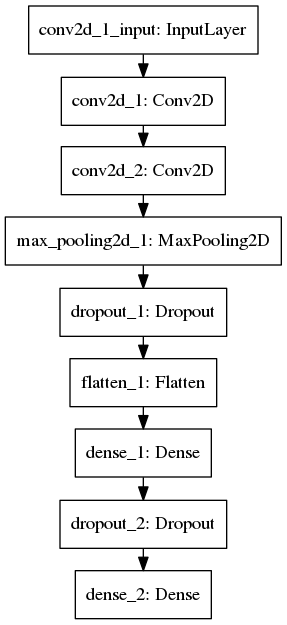
\includegraphics[width=40mm,scale=0.5]{figures/mnist/CNN_model.png}
%\caption{The structure of the CNN used throughput this paper. The final fully connected layer is \textit{softmax} activated while the previous layers are \textit{relu} activated.}
%\end{figure}

The core libraries used were Keras~\cite{chollet2015keras} with a TensorFlow\footnote{https://www.tensorflow.org/} backend for the MNIST CNN. GPFlow~\cite{GPflow2017} was used to implement the Gaussian process model due to its support for large, high dimensional training data\footnote{GPFlow implements sparse variational GPs described in Section~\ref{sec:background:gp} as well as batched training}. Scipy's machine learning toolkit was also tested but was found to be unsuitable.

The models tested are
\begin{enumerate}
\item Keras MNIST CNN trained on 60,000 training images.
\item 3 different GPs trained on features extracted from the CNN's second to last layer.
\item A hybridized model merging CNN and GP predictions, motivated and developed in Section~\ref{sec:mnist:hybridization}.
\end{enumerate} 

The CNN structure is as follows. A convolutional layer with 32 filters, using 3x3 pixel kernels is followed by a 64 channel convolutional layer with 3x3 pixel kernels. This is followed by max pooling with dropout to avoid overfitting. The resulting outputs are flattened into a 1D array and connected to a 128-node layer with dropout. The final layer is a 10-node \textit{softmax} activated fully connected layer. All other layers are \textit{relu} activated.



% * GPFlow, alternatives explored
% * Batching, different GP mechanisms to deal with O(N\^3) scalability
% * Inducing points
% * Approximate trainining time for GP (=> discussion?)
% * Predict time for GP (=> discussion?)


% * Balanced datasets? (! TODO)
% * OPTIONAL: check performance across specific numbers?


% * Hybrid model (=> own Section?)

\section{MNIST}
\label{sec:mnist}
This section focuses on the grayscale MNIST test data set, consisting of 10,000 examples, each 28x28 pixels.

\subsection{Accuracy and Model Motivation}
\label{sec:mnist:acc}

Table~\ref{tab:model_accuracies} shows the test-set accuracy of the CNN, along with three different Gaussian processes: one using a \textit{Polynomial} kernel, one using the \textit{Matern12} kernel, and the last a \textit{Matern32*Linear} kernel (referred to as \textit{combined} kernel from now on). For explanation of the standalone kernels please refer to~\citet{rasmussen2006gaussian}.


\begin{table}[htb]
\caption{MNIST test set accuracy of of various models. The Hybrid model will be developed in Section~\ref{sec:mnist:hybridization}.}
\vskip 0.15in
\begin{center}
\begin{small}
\begin{sc}
\begin{tabular}{lcccr}
\toprule
Model 				& Accuracy \\
\midrule
CNN    				& 99.11\%  \\
Matern12 GP	 		& 99.03\%  \\
Polynomial GP    	& 98.91\%  \\
Linear*Matern32 GP	& \textbf{99.14\%}  \\
Hybrid    			& \textbf{99.14\%}  \\
\bottomrule
\end{tabular}
\end{sc}
\end{small}
\end{center}
\vskip -0.1in
\label{tab:model_accuracies}
\end{table}


%\begin{figure}[hbt]
%\centering
%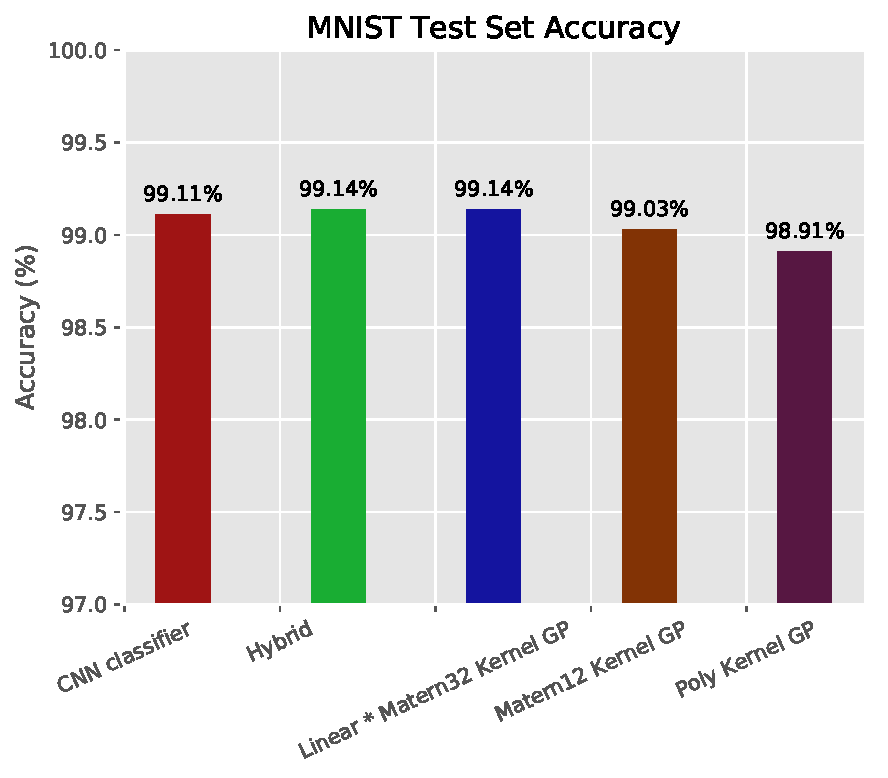
\includegraphics[width=\hsize]{figures/mnist/accuracies.pdf}
%\caption{Accuracy across the different models presented throughout this paper. The Hybrid model will be developed in Section~\ref{sec:mnist:hybridization}. The models perform comparably, except the \textit{Polynomial} kernel which is marginally worse.}
%\label{fig:model_accuracies}
%\end{figure}


It will be shown later that the \textit{Polynomial} kernel performs well in adversarial situations, as does \textit{Matern12}, while the \textit{combined} kernel appears to inherit properties from its two components: \textit{Linear} kernels exhibit strong performance on non-adverserial datasets, while \textit{Matern32} performs worse across the board but is most effective at merging with CNN predictions. This will exploited in  Section~\ref{sec:mnist:hybridization}. Of 17 different single and combined kernels, these had the most interesting properties.

While exploring the GP design space, many configurations were tested. The most influential by far was the number of inducing points used. All kernels in this paper were created using every 25th data point as a possible inducing point and allowed to be automatically optimized during training. Minibatch sizes were set at 8000. A Gaussian noise kernel was added to all kernels with constant variance 0.1, though its inclusion nor its variance have much impact on results. Allowing the GP to optimize a lengthscale parameter per input dimension did not improve performance but increased training time and was left out.

%* CNN performance
%* Show GP performance across various kernels
%* Many configurations were explored, results
% * White noise variance is not a big factor in performance
% * Performance is most correlated with 
%* Explain decision to use Polynomial and Linear*Matern32
% * inherits linear robustness to Blur/Low contrast
% * Inherits nice Matern32 properties for Hybridization
% * not that roboust to adverserial... while Matern12 is

% optional: * footnote SVM as a example of another kernel method

\subsection{Distribution of Variance}

Accuracy is a useful statistic to keep in mind. However, the goal of this paper is to examine the utility of prediction variance, which the CNN does not provide. Figure~\ref{fig:mnist-variances} examines the distribution of variance for correctly, and incorrectly classified examples using the \textit{combined} kernel.


\begin{figure}[hbt]
\centering
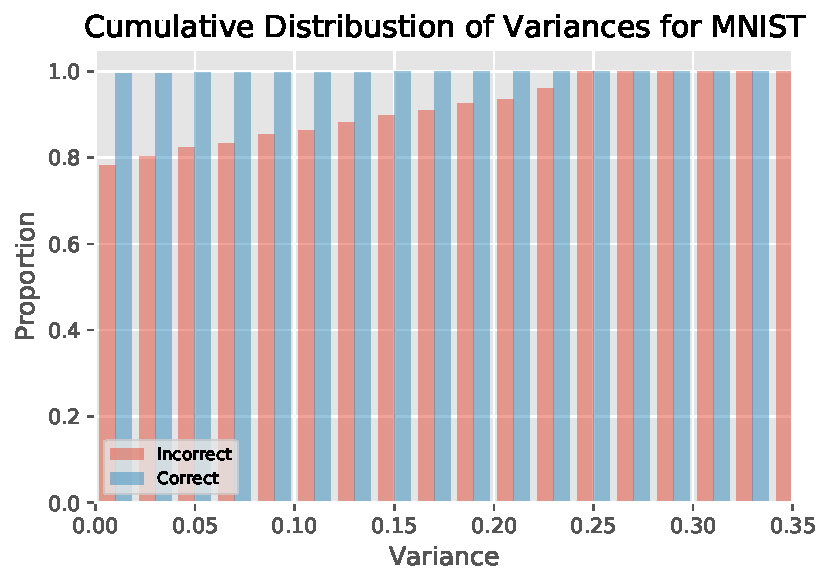
\includegraphics[width=\hsize]{figures/mnist/variances_combined.pdf}
\caption{Distribution of Variances for both incorrect and correctly classified examples.}
\label{fig:mnist-variances}
\end{figure}


This plot clearly shows that the variance of incorrectly predicted classes is skewed higher than when correctly classified. One might expect correct classifications are on average confidently predicted. Indeed, this is supported here, showing inputs that are incorrectly classified have a lower confidence (higher variance). 

%This is a useful property when discussing interpretability: by presenting the variance to human users, a judgement can be made about how much to trust the predicted class, or whether consideration should be given to other predictions that have lower probability but are within, say, a standard deviation of the most likely class.

\subsection{Statistically Significant Predictions}
We can determine statistical significance of predictions by setting some probability $a$ we wish to be sure by. This is usually set to $a=95\%$ confidence. This corresponds to an interval $p \pm 1.96*\sigma$, where $p$ is class probability and $\sigma^2$ is variance. Using this, if the top class's interval does not overlap any other we have a statically significant result.


\begin{table}[h]
\caption{Statistically Significant Predictions on MNIST using 95\% confidence bounds for the \textit{combined} kernel.}
\vskip 0.15in
\begin{center}
\begin{small}
\begin{sc}
\begin{tabular}{lcccr}
\toprule
							&  Combined  	\\
\midrule
\% Significant				& 97.55\%		\\
\% Correct and Significant  & 99.82\%  		\\
\% Incorrect and Not Significant & 28.16\% \\
\bottomrule
\end{tabular}
\end{sc}
\end{small}
\end{center}
\vskip -0.1in
\label{tab:statsig}
\end{table}

From this we can conclude that a user can be extremely sure of statistically significant responses, and should be more weary of insignificant ones, as there is a 28\% of it being incorrect on standard MNIST inputs.

\subsection{SVGP Variance}
\label{sec:svgp-variance}
The GP implementation used in this paper is the sparse variational gaussian process (SVGP) implemented in GPFlow. It is worth double checking that the variance being predicted makes sense and is providing additional information.

\begin{figure}[hbt]
\centering
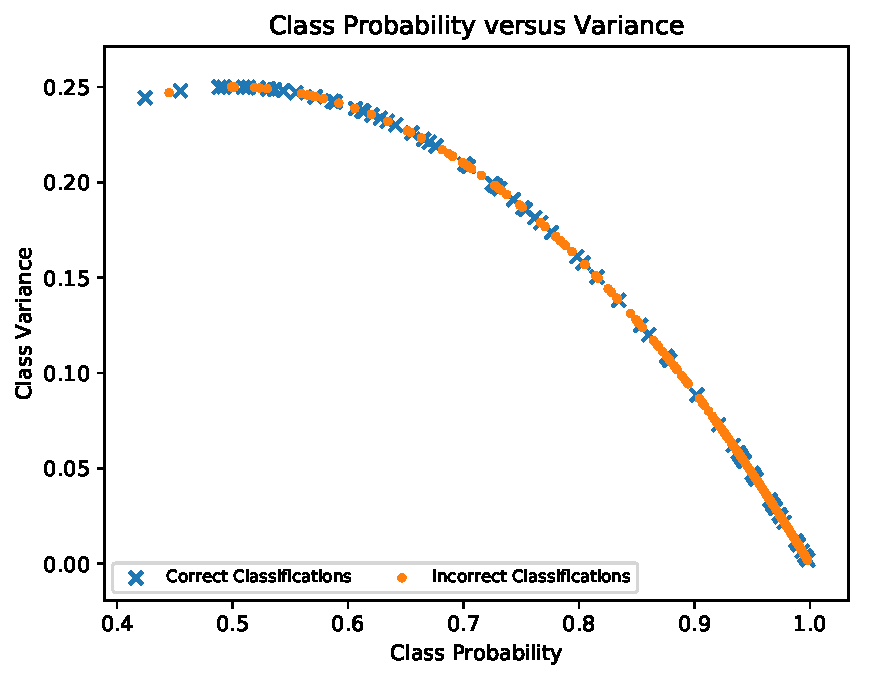
\includegraphics[width=\hsize]{figures/mnist/mu_versus_var_combined.pdf}
\caption{Plotting class probability versus variance on the standard MNIST dataset. They are totally correlated and thus one completely determines the other.}
\label{fig:all_variances}
\end{figure}

The above figure shows that, actually, with this technique and implementation, the class probability completely determines the predicted variance. In fact, a peek into the implementation reveals that variance $\sigma^2$ is calculated from the predicted mean $p$ as $\sigma^2 = p - p^2$.

Note that this observation does not invalidate the usefulness of variance -- it simply says that there is no point getting both mean and variance from the SVGP and analyzing them separately. Calculating the variance and in turn standard deviation is still a useful indicator for explaining results, and later it shall be used to merge \textit{softmax} and GP predictions.

A human operator that did not have this information may try to interpret the class probabilities and variances independently. While not harmful on its own, it could certainly lead to confusion and doubt about the system being presented to them.

It is tempting to calculate variance from CNN predictions in a similar way. However, there is no mathematical reasoning (that I am aware of) that suggests variances calculated this way have any meaning. On the other hand, GPs are accepted as being mathematically sound, so either using $\sigma^2 = p - p^2$ results in proper variance, or GPFlow contains a faulty implementation.

%* Plot GP prediction probability versus confidence
%* Show it's fully deterministic (TODO double check code to make sure it is -- YUP)
%* Conclude variance is not actually extra information but useful for interpretation
%* Discuss interpretability, show some plots (? what plots was i thinking of here TODO)

\subsection{Examining Misclassifications}

I further examine misclassifications on the MNIST dataset, for both CNNs and the \textit{combined} kernel GP.

%\begin{figure}[hbt]
%\centering
%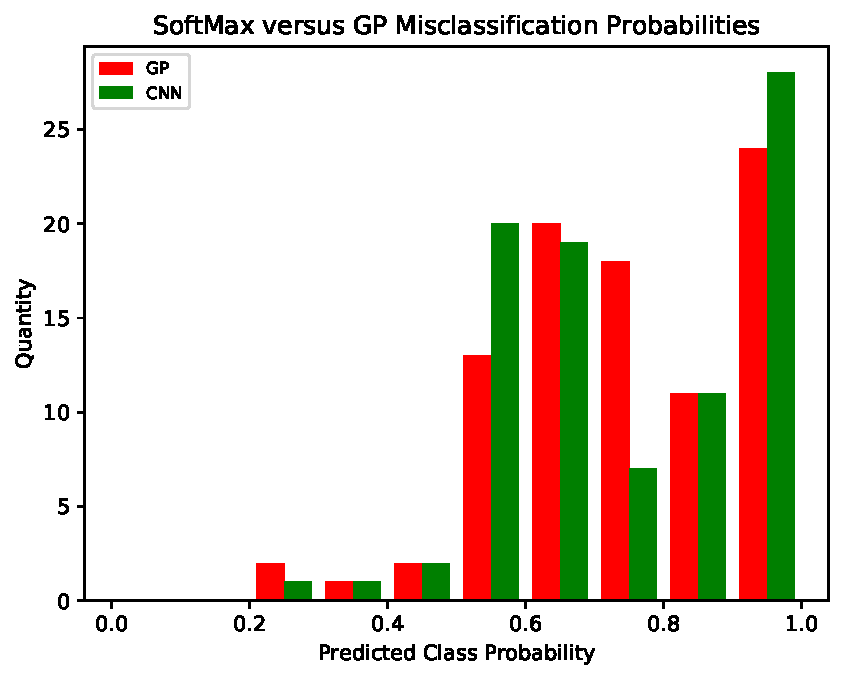
\includegraphics[width=\hsize]{figures/mnist/cnn_vs_gp_misclassification_prob_combined.pdf}
%\caption{Misclassification confidences for CNN and GP with the %\textit{combined} kernel.}
%\label{fig:mispredictions}
%\end{figure}

\begin{table}[htb]
\caption{Mean and Standard Deviation of probability of incorrect predicted classes for the \textit{combined} kernel GP and the CNN.}
\label{tab:misprediction}
\vskip 0.15in
\begin{center}
\begin{small}
\begin{sc}
\begin{tabular}{lcccr}
\toprule
Model			& Mean Probability  	& Standard Deviation  \\
\midrule
GP   			& 74.5\% 		&  17.7\% \\
CNN			 	& 75.3\%		& 18.5\%  \\
\bottomrule
\end{tabular}
\end{sc}
\end{small}
\end{center}
\vskip -0.1in
\label{tab:mispredictions}
\end{table}


From Table~\ref{tab:misprediction} we see that the CNN produces slightly higher probabilities when mis-classifying examples. From this we can loosely conclude that we should put more trust into the GP's prediction probabilities than the CNN's, a fact used later.


%As we established that variance is correlated directly with prediction probability, we expect GPs to have low probabilities when incorrectly predicting results. However, there is no such interpretation for the CNN probabilities, and we can only really conclude that we should put more trust into the GP's prediction probabilities than the CNN's, as the CNN will be confident even in wrong cases.



\begin{figure}[htb]
\centering
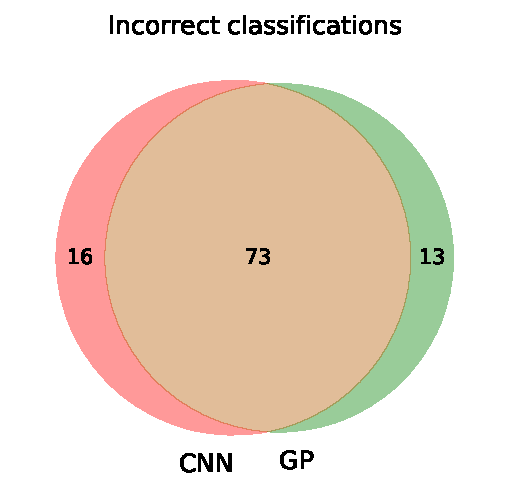
\includegraphics[scale=0.50]{figures/mnist/venn-Linear-Matern32-Kernel-GP.pdf}
\caption{Overlap in misclassifications of the CNN and the \textit{combined} GP model.}
\label{fig:venn}
\end{figure}

The Venn diagram in Figure~\ref{fig:venn} illustrates that both models largely fail on the same 73 test images. These are digits such as the one in Figure~\ref{fig:difficult}, and can be seen as the truly difficult or ambiguous images. Nothing much can be done about them.

\begin{figure}[h!]
\begin{minipage}[c]{.4\hsize}
\centering
\subfloat[Hard Digit]{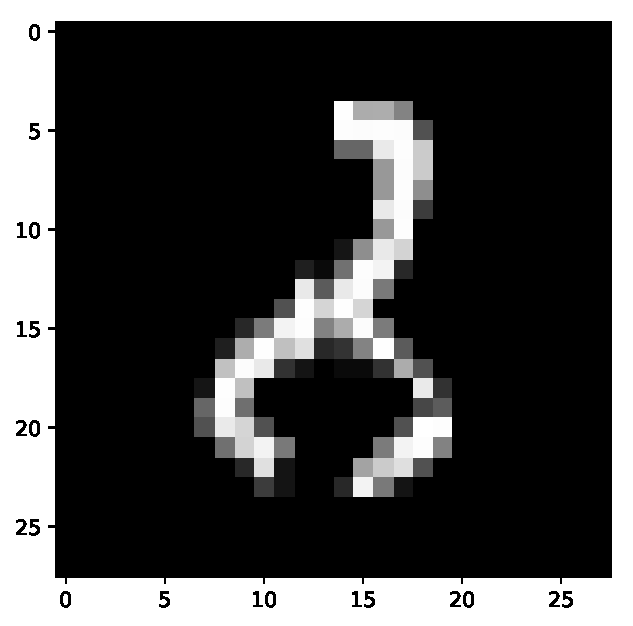
\includegraphics[width=2cm]{figures/mnist/both_incorrect_example_linear.pdf}}
\end{minipage} %
\begin{minipage}[c]{.6\hsize}
\centering
\subfloat[CNN Prediction]{ 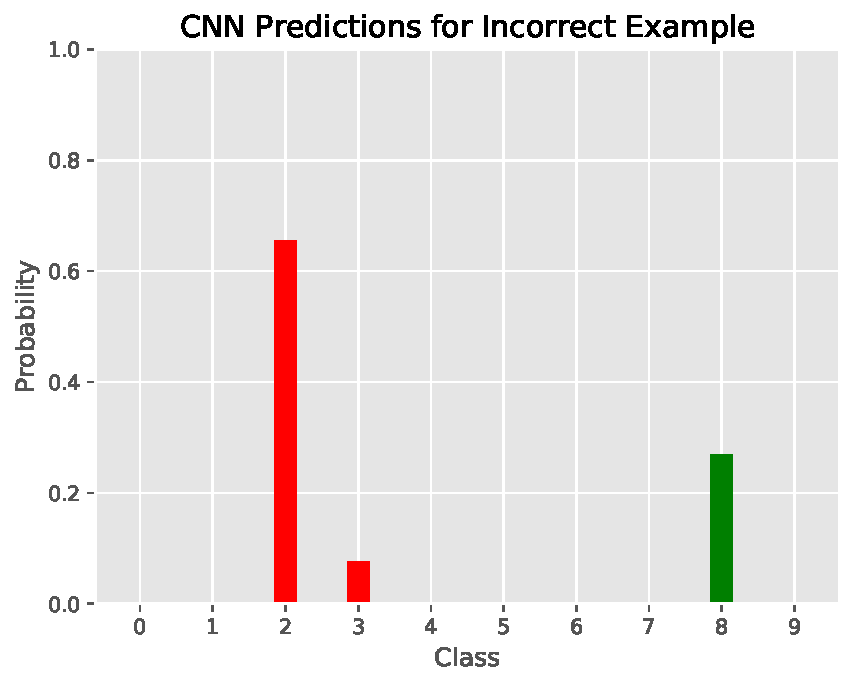
\includegraphics[height=3.5cm]{figures/mnist/both_incorrect_cnn_probs.pdf}}\par

\subfloat[GP Predictions with 1 standard deviation]{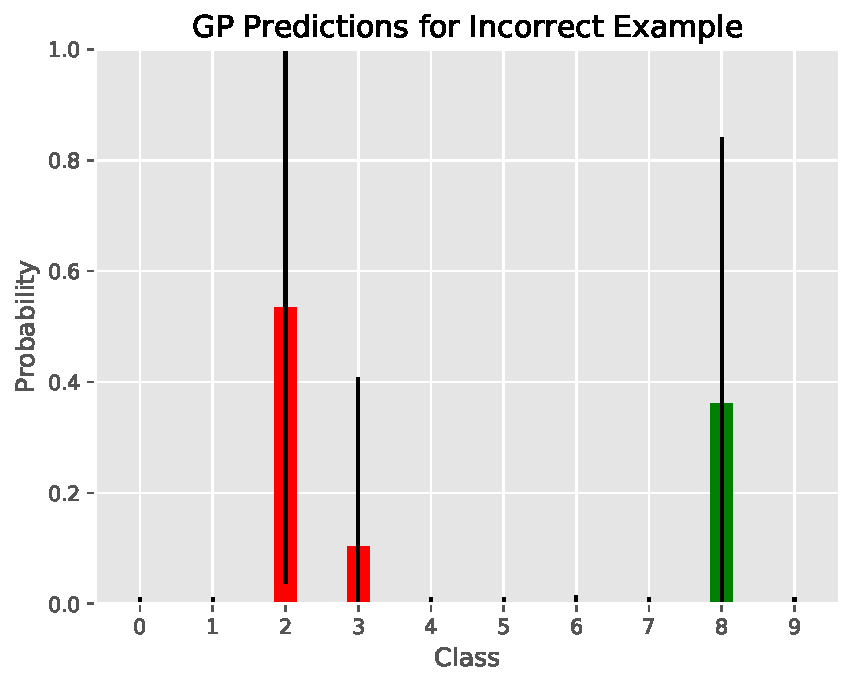
\includegraphics[height=3.5cm]{figures/mnist/both_incorrect_gp_linear_probs.pdf}}
\end{minipage}
\caption{An example of a truly difficult image that both models fail on. The green bar represents the true class, while the tallest red one is the predicted class.}
\label{fig:difficult}
\end{figure}




\begin{figure}[htb]
\begin{minipage}[c]{.49\hsize}
\centering
\subfloat[CNN Misclassified]{
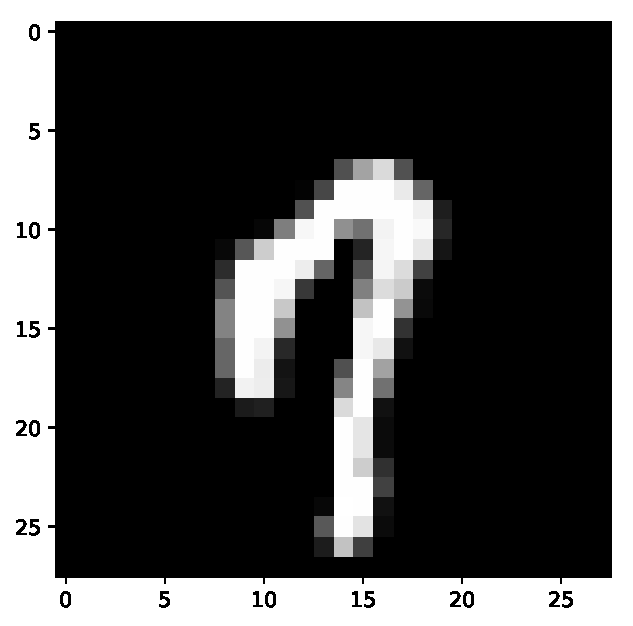
\includegraphics[width=1cm]{figures/mnist/cnn_incorrect_only_example_linear.pdf}}\\

\subfloat[CNN Wrong Predictions]{ 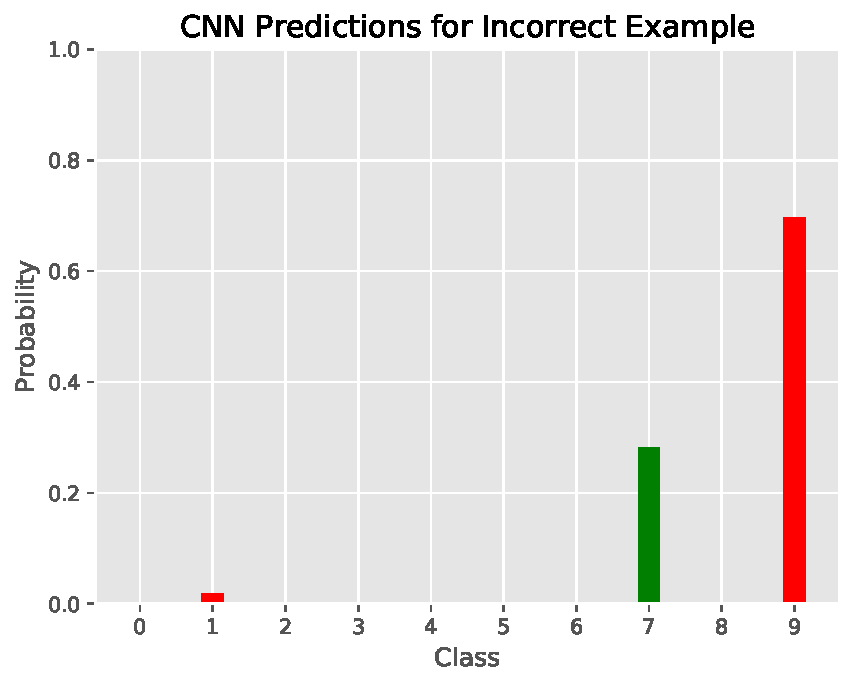
\includegraphics[width=3.95cm]{figures/mnist/cnn_incorrect_only_cnn_probs.pdf}}\\

\subfloat[GP Right Predictions]{
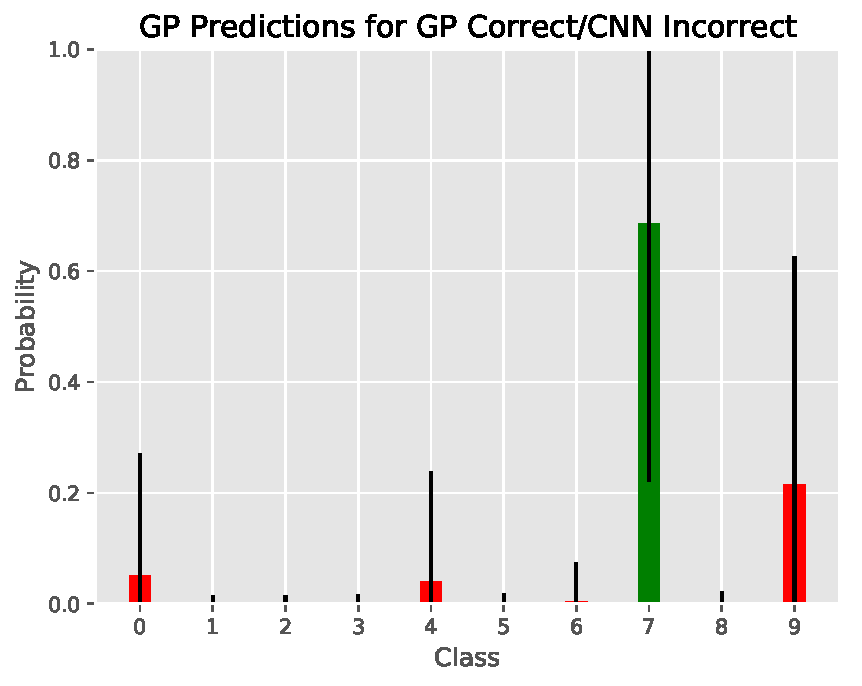
\includegraphics[width=3.95cm]{figures/mnist/cnn_incorrect_only_gp_linear_probs.pdf}}
\end{minipage} %
\vrule{}
\begin{minipage}[c]{.49\hsize}
\centering
\subfloat[GP Misclassified]{
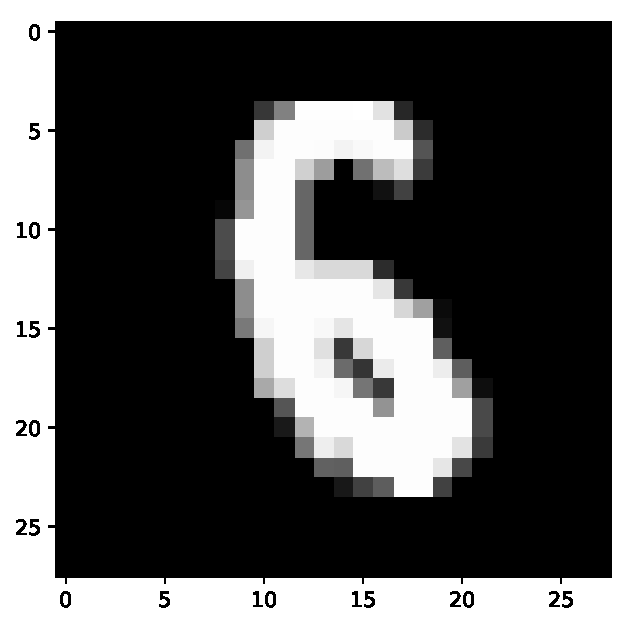
\includegraphics[width=1cm]{figures/mnist/gp_incorrect_only_example_linear.pdf}}\\

\subfloat[CNN Right Predictions]{ 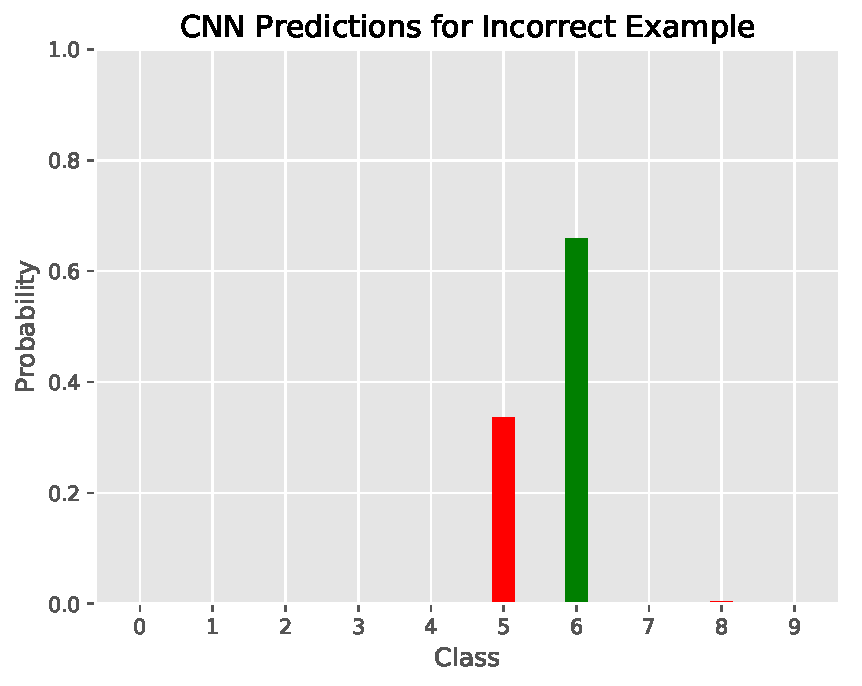
\includegraphics[width=3.95cm]{figures/mnist/gp_incorrect_only_cnn_probs.pdf}}\\

\subfloat[GP Wrong Predictions.]{
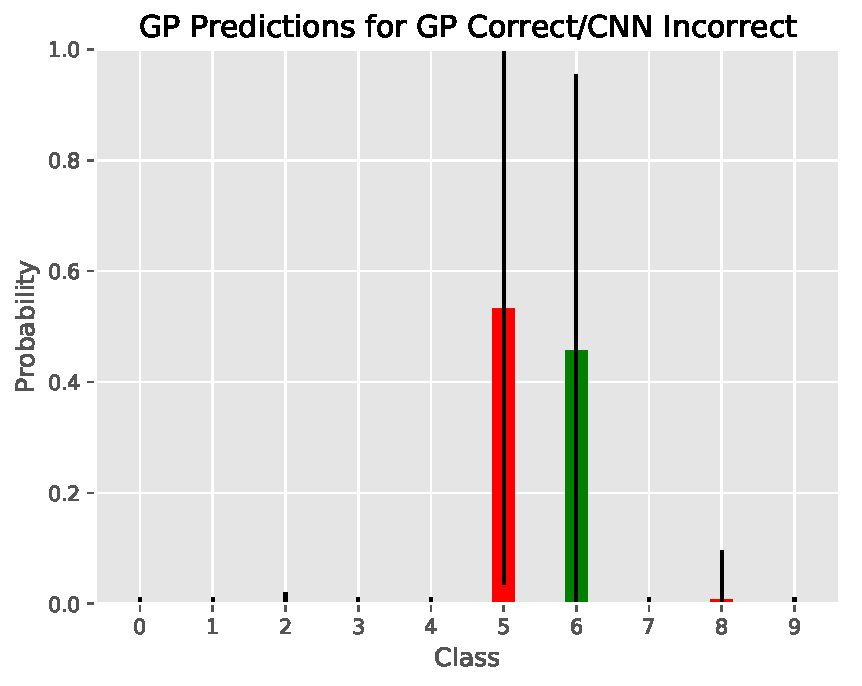
\includegraphics[width=3.95cm]{figures/mnist/gp_incorrect_only_gp_linear_probs.pdf}}
\end{minipage} %
\caption{Examining cases of misclassifications. The left column corresponds to one of the 16 examples the CNN classified incorrectly, while the right column stems from the GP's incorrect classifications. With the right heuristic these case, and others, may be salvageable.}
\label{fig:mnist:mismatch}
\end{figure}

However, more interesting is the non-overlapping region of the Venn diagram. From Figure~\ref{fig:mnist:mismatch} we see there is hope for boosting accuracy by combining the results from the CNN and the GP: the true class, in green, has a high probability but is not the highest. This inspires the hybridized model in the next section.

% * Plot CNN and GP mis-prediction probabilities
%  * Discuss... conclusion is that CNN more confidently mis-predicts results?
% * Show examples that both fail, one fails
% * Discuss that nothing can be done when both fail - no extra information
% * Show overlap, non-overlap in misclassifications
% * Inspires Hybridization!

\subsection{Hybridization}
\label{sec:mnist:hybridization}

Because we have a (small) ensemble of classifiers when using both the CNN and a GP, a disagreement amounts to an extra bit of information. We can try to choose the best result, steered by the variance predicted by the GP. The driving principle in this heuristic is that we trust the Gaussian process model more than the CNN.

\subsubsection{Algorithm}
\label{sec:mnist:hybridization:criteria}

When merging CNN and GP predictions, we default to the GP prediction, only choosing the CNN's result if the following conditions hold:

\begin{enumerate}
\item The CNN's top prediction is within $d$ standard deviations of the corresponding GP's probability (calculated using corresponding GP variance). This ensures that the GP agrees the CNNs prediction is plausible. 
\item The CNN's top prediction is within $d$ standard deviations of the top GP's prediction (calculated using top GP variance).
\item The GP's top prediction is not $d$ or more standard deviations from the GP's corresponding prediction.
\end{enumerate}

The first condition pulls the GP accuracy toward the CNN to either increase or decrease total accuracy. The latter two conditions mitigate worsened accuracy to an extent, ensuring that the GP's decision is accepted when it is very confident compared to the CNN and that the CNN's probability isn't too low, even if plausible according to the GP. 

\subsubsection{Discussion}
When accepting a CNN prediction, we lose a meaningful variance and the resulting insight a human might utilize. However this could easily be fixed by flagging the result as uncertain, due to disagreement, as well as presenting the GP predictions. 

Secondly, in this situation some kernels boost accuracy more than others. I believe this stems from larger non-overlapping regions as compared to the Venn diagram presented before. Through experimentation the \textit{Matern32}, and in turn the combined \textit{Linear*Matern32}, kernels were found to provide the best results. 

Lastly, assuming the CNN and the GP outputs are available this cheap: linear in the number of classes.

From here on I also present hybridized model results using the \textit{combined} kernel with an acceptance criteria of $d=0.2$ standard deviations. 



\begin{table*}[t]
\caption{Accuracy across all models and n-MNIST data sets.}
\vskip 0.15in
\begin{center}
\begin{small}
\begin{sc}
\begin{tabular}{lcccr}
\toprule
Model 				& AWGN 	& Motion Blur	& Low Contrast + AWGN \\
\midrule
CNN    				& 95.38\% 		&	 94.58\%		& 77.15\%   \\
Matern12 GP	 		& 96.10\%		& 87.46\%			& 71.52\%    \\
Polynomial GP    	& 95.68\%		& 93.39\%		& \textbf{81.18}\%  	  \\
Linear*Matern32 GP	& 96.13\%		& 94.61\% 			& 78.95\%   \\
Hybrid    			& \textbf{96.19}\%		& \textbf{94.71}\% 	& \textit{79.27}\%   \\
\bottomrule
\end{tabular}
\end{sc}
\end{small}
\end{center}
\vskip -0.1in
\label{tab:nmnist:accuracies}
\end{table*}

\section{n-MNIST}

The `noisy'-MNIST dataset stems from~\citet{basu2017learning}. The authors provide three transformations of the MNIST images: added white noise, motion blurred, and lowered contrast and white noise.

\begin{figure}[htb]
\centering
\subfloat[]{
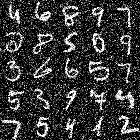
\includegraphics[width=0.3\hsize]{./images/awgn_95.png}
}
\centering
\subfloat[]{
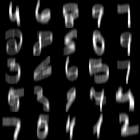
\includegraphics[width=0.3\hsize]{./images/motion_blur_15_5.png}
}
\centering
\subfloat[]{
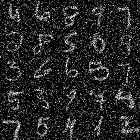
\includegraphics[width=0.3\hsize]{./images/contrast_2_12.png}}

\caption{Added white noise, motion blurred, and low contrast + white noise samples. Images from \url{http://csc.lsu.edu/~saikat/n-mnist/}}
\end{figure}



\subsection{Accuracy}


Table~\ref{tab:nmnist:accuracies} shows how each model performs across the different n-MNIST datasets. The hybrid model consistently outdoes the standard \textit{Linear * Matern32} kernel by a small amount. It is reassuring to note that the heuristic devised is not harming performance, and boosting it by 0.3\% in the best case.


%\begin{figure}[h]
%\centering
%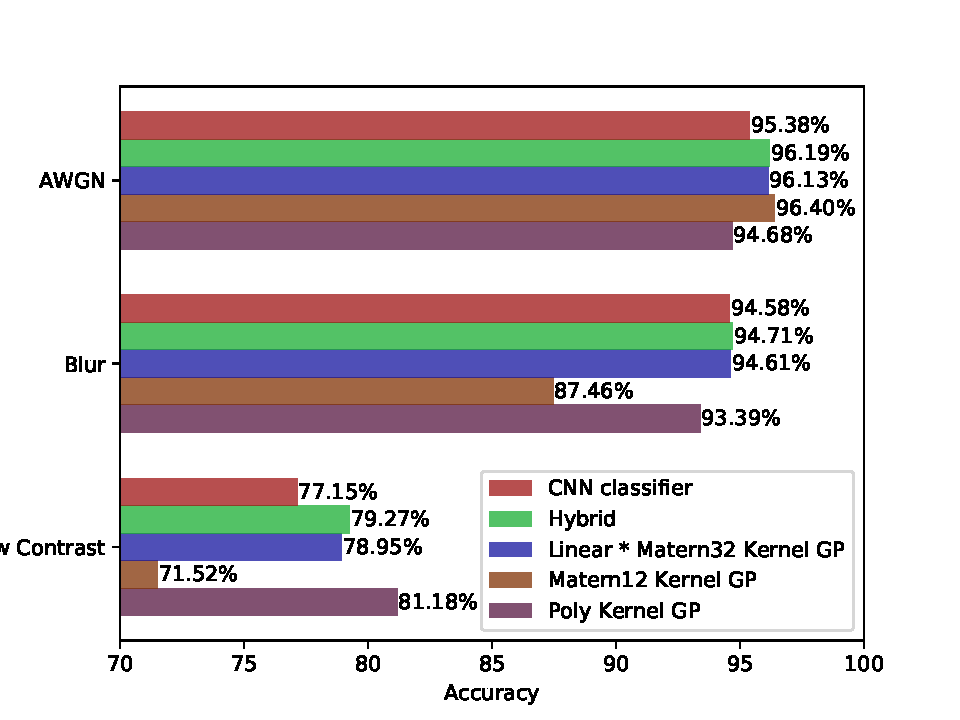
\includegraphics[width=\hsize]{figures/nmnist/all_accuracies.pdf}
%\caption{Performance across all models and n-MNIST data sets.}
%\label{fig:nmnist:accuracies}
%\end{figure}

Most kernels outperform the CNN excepting \textit{Matern12}. This kernel allows quite a lot of movement, i.e. the covariance between close data points is low, so it is possible it overfits the training data and suffers in very different situations.

From this experiment, it is quite evident that each kernel has some strengths, and none of them outperform the others across the board. This could be the basis of larger ensemble methods, and an idea discussed in Section~\ref{sec:discussion}.

\subsection{Distribution of Standard Deviations}

The distribution of variances on the various n-MNIST test sets are as expected, with Figure~\ref{fig:nmist:vars} showing the correct examples having much lower variance in general than the incorrect examples, though on more difficult datasets, such as the low contrast + white noise version, the distributions become more and more similar.

\begin{figure}[h!]
\centering
\subfloat[With white noise]{
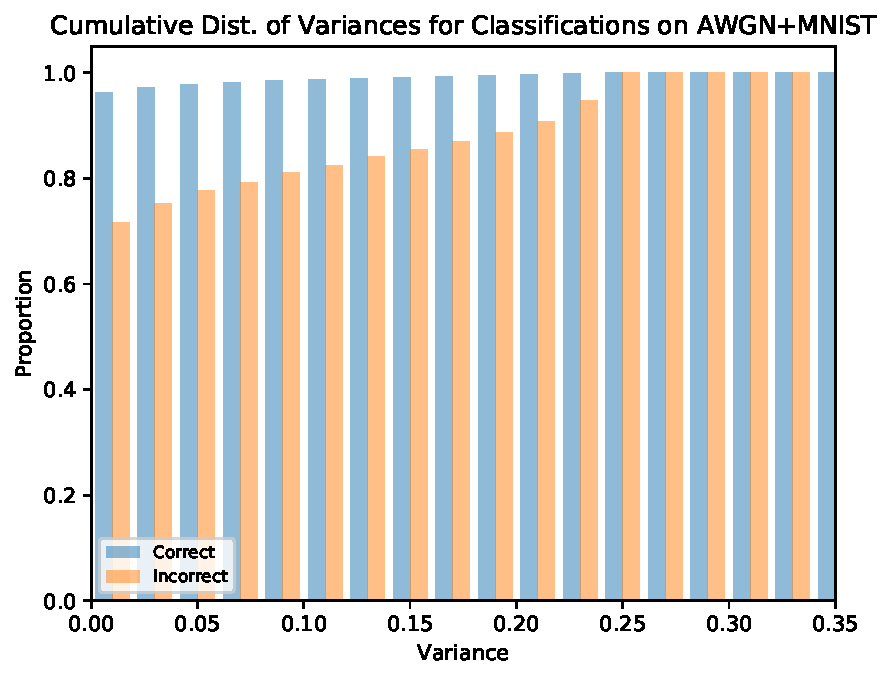
\includegraphics[width=\hsize]{./figures/nmnist/awgn_variances_combined.pdf}
}

\centering
\subfloat[With motion blur]{
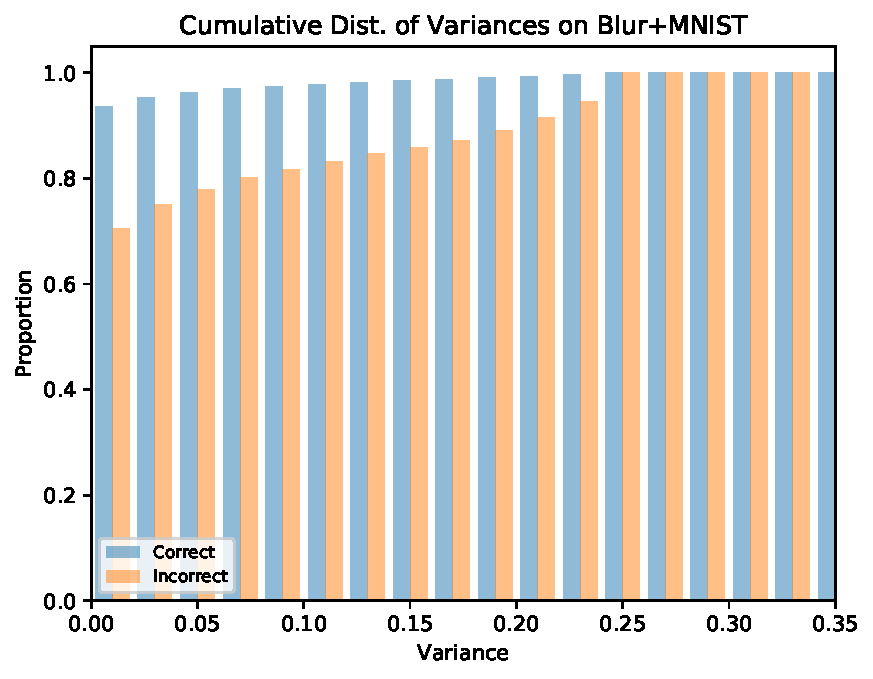
\includegraphics[width=\hsize]{./figures/nmnist/blur_variances_combined.pdf}
}

\centering
\subfloat[Low contrast and with white noise]{
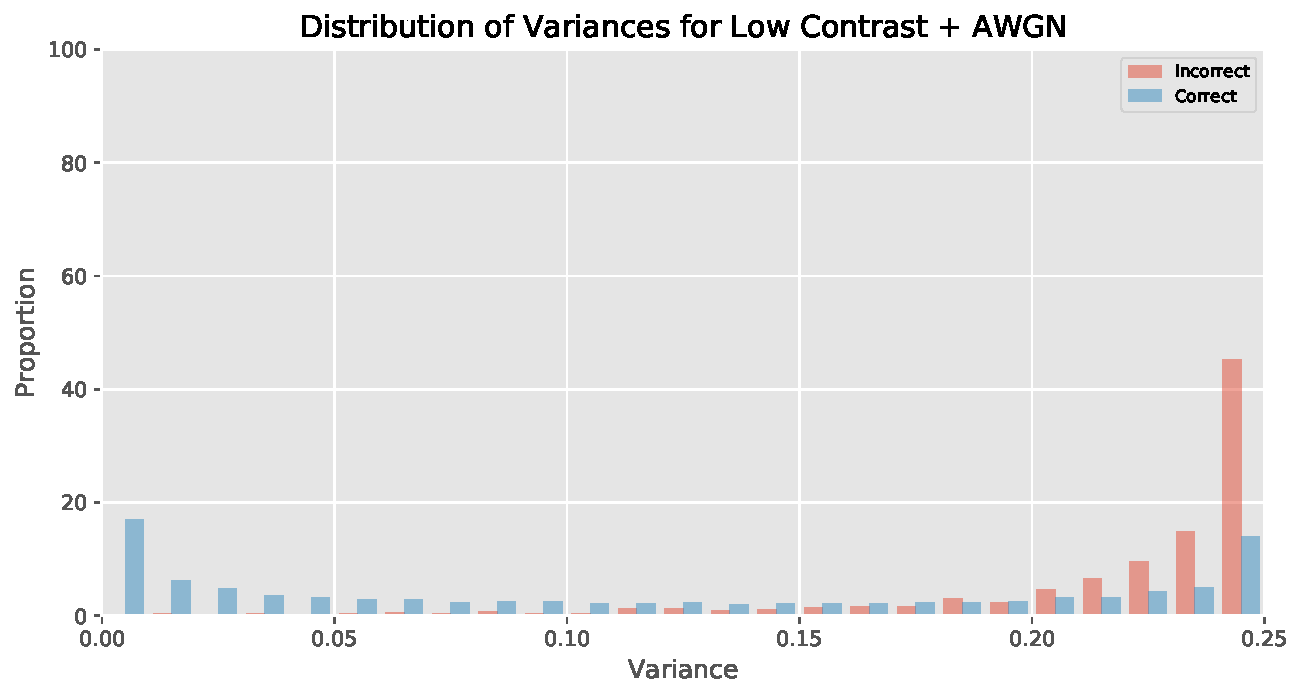
\includegraphics[width=\hsize]{./figures/nmnist/lowcontrast_variances_combined.pdf}}

\caption{Variances across the n-MNIST dataset}
\label{fig:nmist:vars}
\end{figure}



\section{Adverserial Attacks}
\label{sec:adversarial}
Adverserial attacks are described in Section~\ref{sec:background:adv}. Cleverhans~\cite{papernot2017cleverhans} generates perturbations using FGSM on the 10,000 MNIST images via the trained CNN.

\begin{table}[htb]
\caption{Mean and Standard Deviation of probability of incorrect predicted classes for the \textit{combined} kernel GP and the CNN.}
\vskip 0.15in
\begin{center}
\begin{small}
\begin{sc}
\begin{tabular}{lcccr}
\toprule
Model 				& Accuracy \\ 				
\midrule
CNN    				& 62.16\%  \\
Matern12 GP	 		& 64.14\%  \\
Polynomial GP    	& \textbf{65.67}\%  \\
Linear*Matern32 GP	& 62.58\%  \\
Hybrid    			& 62.47\%  \\
\bottomrule
\end{tabular}
\end{sc}
\end{small}
\end{center}
\vskip -0.1in
\label{tab:adv:accuracies}
\end{table}

%\begin{figure}[htb]
%\centering
%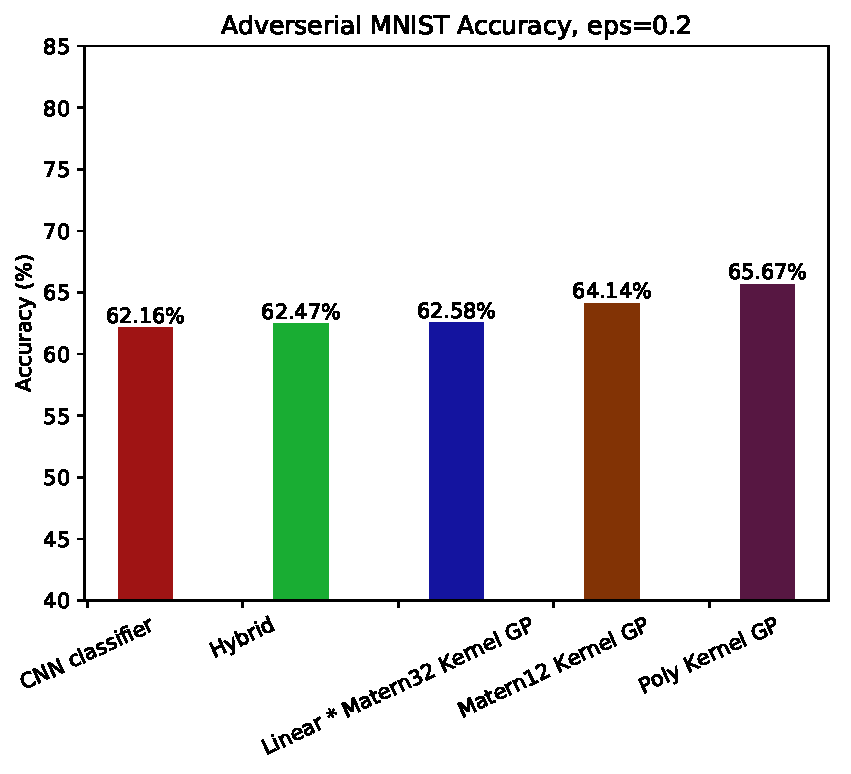
\includegraphics[width=\hsize]{./figures/adversarial/accuracies_eps02.pdf}
%\caption{Accuracies on FGSM perturbed MNIST, $\epsilon=0.2$}
%\label{fig:adv:accuracies}
%\end{figure}

Using an $\epsilon=0.2$, all the models show large performance degradations from the 99\% accuracy presented in Section~\ref{sec:mnist:acc}.  Returning to analyzing 95\% confident predictions, we see in Table~\ref{tab:adv_statsig}, we can see that adversarial attacks produce a large number of very confident incorrect predictions, successfully confusing the GP as well as the CNN.

\begin{table}[h]
\caption{Statistically Significant Predictions on Perturbed MNIST using 95\% confidence bounds.}
\vskip 0.15in
\begin{center}
\begin{small}
\begin{sc}
\begin{tabular}{lcccr}
\toprule
							&  Combined  	\\
\midrule
\% Significant				& 51.39\%		\\
\% Correct and Significant  & 72.43\%  		\\
\% Incorrect and Not Significant & 47.82\% \\
\bottomrule
\end{tabular}
\end{sc}
\end{small}
\end{center}
\vskip -0.1in
\label{tab:adv_statsig}
\end{table}



\subsection{Varying $\epsilon$}
Previous work by \citet{Bradshaw2017} showed that for GPDNNs, which have GP's trained end to end with CNNs from scratch, targeting the plain CNN architecture does not harm the GPDNN much. This conclusion is rather obvious since they learn different structure. Vice versa, their CNN is resistant to attacks on the GPDNN.

\begin{figure}[h!]
\centering
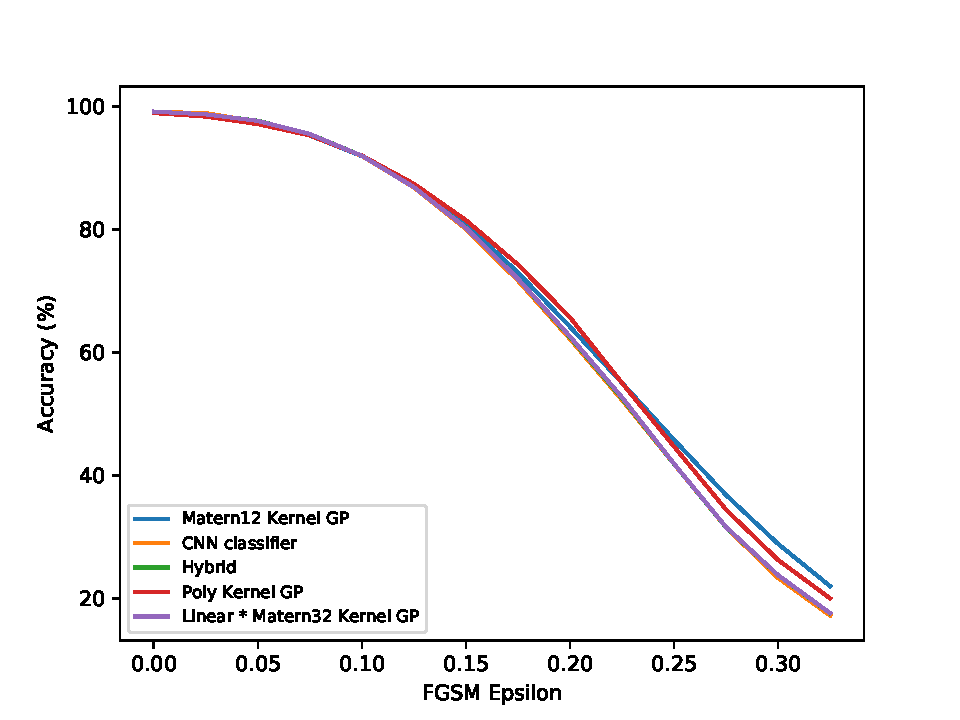
\includegraphics[width=\hsize]{./figures/adversarial/epsilons.pdf}
\caption{Classification Accuracies on FGSM attacked MNIST images across varying $\epsilon$}
\label{fig:adv:epsilons}
\end{figure}

Figure~\ref{fig:adv:epsilons} shows, in the best case with \textit{Polynomial} or \textit{Matern12} kernels, at most 5-10\% boosts can be expected as $\epsilon$ becomes large, but generally GPs degrade just as much as the CNN. Thus, GPs do not provide the hoped resistance to adversarial attacks. This is rather sensible since most of the CNN structure is shared between models and producing features for the GP that appear like other classes with high confidence. 

\section{Discussion}
\label{sec:discussion}

The best presented use of variance is to identify statistically significant predictions, which users can trust to an extremely high degree. For instance, a system could a statistical test to flag uncertain results for further inspection. This is especially useful in situations where false negatives are costly, such as in the medical field. 

As noted in Section~\ref{sec:svgp-variance}, in this implementation variance is actually just as informative as class probability. This does not mean variance is useless information since we can use it for inter-class statistical tests, as well as presenting it to human users who can easily reason in terms of standard deviations.

An alternative use of variance, the hybridizing approach, was found to provide incremental gains over the \textit{Linear * Mater32} kernel. Unfortunately, it also slightly worsened performance in adversarial situations. It is possible that more consistent accuracy gains are within reach with more sophisticated methods. One obvious approach is to further refine the acceptance criteria described in Section~\ref{sec:mnist:hybridization:criteria}, or experiment with different acceptance parameter values, or even using 3 different parameters, one for each part of the criterion. However, none of these are likely to lead to particularly novel algorithms or dramatically improved results. Even worse, all examples that were rescued with the hybridized approach turned out to be statistically insignificant predictions, so this approach is not useful at all if using statistical tests to eliminate bad predictions in the first place.

As a positive, if only trying to marginally increase accuracy, creating the hybridization is almost free: most of the CNN needs to be evaluated to extract features to feed into the GP. For instance, in TensorFlow, executing the entire CNN and saving an intermediate value incurs almost no cost. If the Gaussian process is going to be executed in $O(n^2)$ anyway, the hybridization is only $O(m)$ (for $m$ classes) more expensive.

Whether training the GP at all is worth it is another question: even with sparse variational implementations, GPs still do not scale as well as CNNs, and this investigation has revealed that classification accuracy is generally on par or only slightly better than CNNs. In situations where interpretation is important, it is worth re-evaluating the entire training set to train the GP. However, if interpretability is not a concern, I argue using a GP is not useful. 

GPs are also detrimental when dealing with large scale datasets and time-bound execution. A small CNN can be made to execute quickly and at a constant speed regardless of training data size -- GPs predict quadratically in the number of training samples, and even with variational methods are slow to train.

\section{Future Work}

\subsection{Ensembles}
Hybridization between a single GP and a CNN ultimately provides unimpressive results. A more interesting idea could be take the entire process a step further: hybridize based on a multitude of kernels, effectively forming an ensemble. 

As mentioned before, each kernel appears to have different strengths, and it may be possible to come up with a heuristic for merging many predictions. Part of such an investigation would be to explore the role of variance. More heuristics could be developed, or reinforcement learning could be used to decide on an optimal decision strategy, though this would be biased toward its training data and be difficult to generalize.

Finally, this entire investigation depends critically on a closed set of examples to perform well (i.e. we expect that all examples actually belong to one of the 10 classes). The introduction hinted that since softmax strongly accentuates small differences between prediction probabilities, and does not take into account absolute activation of the final layer, CNNs can return high probabilities for examples that are not any of the expected classes. I expect GPs can also be made to exhibit such behavior. This is related strongly to the research area of open set classification~\cite{scheirer2013toward}. Using an ensemble including classifiers specifically trained on irrelevant data could lead to an effective rejection mechanism.

\subsection{Automatic Kernel Building}
It was shown in Section~\ref{sec:adversarial} that kernels have varying adversarial resistance. Another investigative avenue could thus be automatically creating the best kernel for both a data set and adversarial resistance. Automatic kernel choice is already an active research area (for example~\cite{abdessalem2017automatic}, \cite{duvenaud2014automatic}), but without the adversarial effects taking into account. Further, it might be interesting to consider creating kernels that can effectively be ensembled together, i.e. err on maximally different parts of the same dataset.

\section{Conclusion}

This paper examined the utility of variance in classification. To do this, a CNN was trained on the MNIST dataset, and compared to various Gaussian processes on a variety of datasets. The main benefit of variance is interpretability: having access to an uncertainty in a prediction means consumers of classifications can make further judgements about results and don't need to accept predictions at face value; statistical tests can be used to make principled decisions about significant of data.

This paper also presented the idea of merging predictions from the base CNN and the GP, using variance as a guide for choosing one decision of the other. A heuristic was presented which achieved slightly increased test set accuracy on non-adversarial examples. Overall however, a simple two-way merge does not yield impressive results, and a further investigation could be conducted into ensembling multiple different gaussian processes, also steered by prediction variances.

\subsection{Software and Data}

Code, results, and this report can be found at:

\url{https://github.com/flyingsilverfin/CNN_GP_MNIST}

Please note that intermediate results are not saved but can be recomputed, and that some of the configurations are specific to the development machine. % TODO update README on GitHub


\bibliography{gp_cnn_bibliography.bib}
\bibliographystyle{icml2018}



%%%%%%%%%%%%%%%%%%%%%%%%%%%%%%%%%%%%%%%%%%%%%%%%%%%%%%%%%%%%%%%%%%%%%%%%%%%%%%%
%%%%%%%%%%%%%%%%%%%%%%%%%%%%%%%%%%%%%%%%%%%%%%%%%%%%%%%%%%%%%%%%%%%%%%%%%%%%%%%
% DELETE THIS PART. DO NOT PLACE CONTENT AFTER THE REFERENCES!
%%%%%%%%%%%%%%%%%%%%%%%%%%%%%%%%%%%%%%%%%%%%%%%%%%%%%%%%%%%%%%%%%%%%%%%%%%%%%%%
%%%%%%%%%%%%%%%%%%%%%%%%%%%%%%%%%%%%%%%%%%%%%%%%%%%%%%%%%%%%%%%%%%%%%%%%%%%%%%%
\appendix

\end{document}


% This document was modified from the file originally made available by
% Pat Langley and Andrea Danyluk for ICML-2K. This version was created
% by Iain Murray in 2018. It was modified from a version from Dan Roy in
% 2017, which was based on a version from Lise Getoor and Tobias
% Scheffer, which was slightly modified from the 2010 version by
% Thorsten Joachims & Johannes Fuernkranz, slightly modified from the
% 2009 version by Kiri Wagstaff and Sam Roweis's 2008 version, which is
% slightly modified from Prasad Tadepalli's 2007 version which is a
% lightly changed version of the previous year's version by Andrew
% Moore, which was in turn edited from those of Kristian Kersting and
% Codrina Lauth. Alex Smola contributed to the algorithmic style files.
